
\subsubsection{Licence}
Contrairement à ce qu'indiquait la page Wikipédia la licence n'est pas \enquote{GNU GPL
modifiée} mais la \enquote{MIT open source license} qui n'existe pas dans la liste GNU
\cite{ref2} mais qu'on peut tout de même retrouver sous le nom de \enquote{The MIT
License} sur le site de l'Open Source Initiative. Je ne l'ai pas retrouvée sur le
site du MIT et il n'y a pas de contact !\\

Les 4 lignes (en verbatim) du site de l'Open Source Initiative :
\begin{verbatim}
Begin license text.

Copyright <YEAR> <COPYRIGHT HOLDER>

Permission is hereby granted, free of charge, to any person obtaining a copy of this software and associated documentation files (the "Software"), to deal in the Software without restriction, including without limitation the rights to use, copy, modify, merge, publish, distribute, sublicense, and/or sell copies of the Software, and to permit persons to whom the Software is furnished to do so, subject to the following conditions:

The above copyright notice and this permission notice shall be included in all copies or substantial portions of the Software.

THE SOFTWARE IS PROVIDED "AS IS", WITHOUT WARRANTY OF ANY KIND, EXPRESS OR IMPLIED, INCLUDING BUT NOT LIMITED TO THE WARRANTIES OF MERCHANTABILITY, FITNESS FOR A PARTICULAR PURPOSE AND NONINFRINGEMENT. IN NO EVENT SHALL THE AUTHORS OR COPYRIGHT HOLDERS BE LIABLE FOR ANY CLAIM, DAMAGES OR OTHER LIABILITY, WHETHER IN AN ACTION OF CONTRACT, TORT OR OTHERWISE, ARISING FROM, OUT OF OR IN CONNECTION WITH THE SOFTWARE OR THE USE OR OTHER DEALINGS IN THE SOFTWARE.
End license text. 
\end{verbatim}

Elle semble un peu \enquote{fantoche}.\\

Sur le site de freertos :
\begin{verbatim}
Permission is hereby granted, free of charge, to any person obtaining a copy of
this software and associated documentation files (the "Software"), to deal in
the Software without restriction, including without limitation the rights to
use, copy, modify, merge, publish, distribute, sublicense, and/or sell copies of
the Software, and to permit persons to whom the Software is furnished to do so,
subject to the following conditions:

The above copyright notice and this permission notice shall be included in all
copies or substantial portions of the Software.

THE SOFTWARE IS PROVIDED "AS IS", WITHOUT WARRANTY OF ANY KIND, EXPRESS OR
IMPLIED, INCLUDING BUT NOT LIMITED TO THE WARRANTIES OF MERCHANTABILITY, FITNESS
FOR A PARTICULAR PURPOSE AND NONINFRINGEMENT. IN NO EVENT SHALL THE AUTHORS OR
COPYRIGHT HOLDERS BE LIABLE FOR ANY CLAIM, DAMAGES OR OTHER LIABILITY, WHETHER
IN AN ACTION OF CONTRACT, TORT OR OTHERWISE, ARISING FROM, OUT OF OR IN
CONNECTION WITH THE SOFTWARE OR THE USE OR OTHER DEALINGS IN THE SOFTWARE.
\end{verbatim}

En approfondissant, il semble que la GNU GPL modifiée ait bien été la licence du
projet jusqu'à son acquisition par Amazon.\\

Pourquoi ont-ils enlevé la première ligne (copyright) ? Ce changement de licence
est-il bien légal ?\\

On peut quand même la retrouver sur gnu.org\cite{ref2} sous le nom de
\enquote{Licence Expat}.

\subsubsection{Code source}
Dépot GIT : \url{https://github.com/freertos/freertos}.\\

Le code est propre et commenté (sans doxygen), assez proche des \enquote{GNU Coding
Standards}\cite{ref4} à première vue.\\

{\small
\begin{verbatim}
The core FreeRTOS source files (those that are common to all ports, but not the port
layer) conform to the MISRA coding standard guidelines.
\end{verbatim}
}
%\\\\
%\enquote{En 2017, le projet et son équipe de \textbf{développeurs} ont été \textbf{acquis par Amazon}}\cite{ref6}.

\subsubsection{Plateformes cible}
Nombreuses dont ARM\_CM7 mais pas spécifiquement la Nucleo-F746ZG.
%\\\\
%\enquote{En 2017, le projet et son équipe de \textbf{développeurs} ont été \textbf{acquis par Amazon}}\cite{ref6}.


\subsubsection{Communauté}
Le site internet \url{https://www.freertos.org/} comporte 5 pages :
\begin{itemize}
	\item Kernel ;
	\item Libraries ;
	\item Resources ;
	\item Community ;
	\item Support.
\end{itemize}

Il n'y a pas de page "License" ce qui montre que l'éthique n'est pas au cœur de
leurs préoccupations.\\

La page d'accueil arbore une magnifique bannière commerciale :
\begin{figure}[!h]
	\begin{center}
		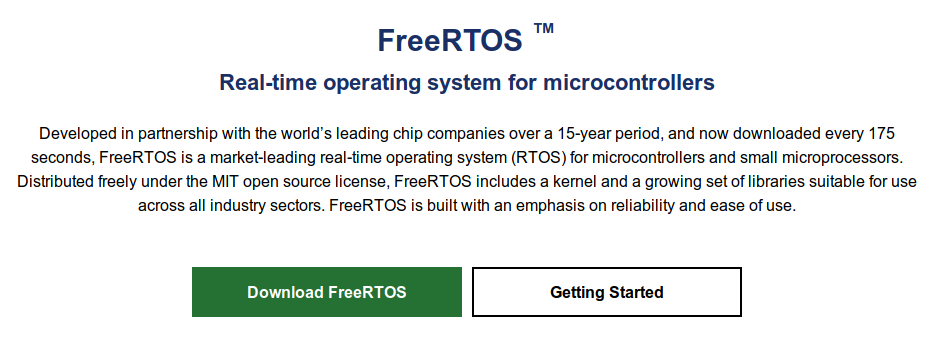
\includegraphics[scale=.5]{images/accueil_site.png}
	\end{center}
\end{figure}

Sur mon affichage aux couleurs inversées, le rose du bouton \enquote{Download
FreeRTOS} est très sexy !\\

Le dépot github indique à ce jour 2774 commits (le dernier il y a 7 jours et 10
contributeurs.
%\\\\
%\enquote{En 2017, le projet et son équipe de \textbf{développeurs} ont été \textbf{acquis par Amazon}}\cite{ref6}.

\subsubsection{Acceptabilité}
\begin{tabular}{lll}
\toprule
	Critère				&	Validé		&	Commentaire	\\
\midrule
	Licence				&	oui			&	historique bancal	\\
	Code source			&	oui			&		\\
	Plateformes cible	&	oui			&	ARM\_CM7	\\
	Communauté			&	oui			&		\\
\bottomrule
\end{tabular}

